% Encoding: UTF-8
%%%%%%%%%%%%%%%%%%%%%%%%%%%%%%%%%%%%%%%%%%%%%%%%%%%%%%%%%%%%%%%%%%%%%%%%%%%%%%%

%%%%%%%%%%%%%%%%%%%%%%%%%%%%%%%%%%%%%%%%%%%%%%%%%%%%%%%%%%%%%%%%%%%%%%%%%%%%%%%
% $Id: slides.tex 17 2011-02-10 15:21:56Z klugeflo $
%%%%%%%%%%%%%%%%%%%%%%%%%%%%%%%%%%%%%%%%%%%%%%%%%%%%%%%%%%%%%%%%%%%%%%%%%%%%%%%

%%%%%%%%%%%%%%%%%%%%%%%%%%%%%%%%%%%%%%%%%%%%%%%%%%%%%%%%%%%%%%%%%%%%%%%%%%%%%%%
%%
%% Vorlage fuer LaTeX-Beamer
%% gemaess dem Corporate Design der Uni Augsburg
%%
%%%%%%%%%%%%%%%%%%%%%%%%%%%%%%%%%%%%%%%%%%%%%%%%%%%%%%%%%%%%%%%%%%%%%%%%%%%%%%%
%%
%% Changelog:
%%
%% 11/02/10 (FAK) Start
%%
%%%%%%%%%%%%%%%%%%%%%%%%%%%%%%%%%%%%%%%%%%%%%%%%%%%%%%%%%%%%%%%%%%%%%%%%%%%%%%%


%%%%%%%%%%%%%%%%%%%%%%%%%%%%%%%%%%%%%%%%%%%%%%%%%%%%%%%%%%%%%%%%%%%%%%%%%%%%%%%

\documentclass[xcolor=pdftex,dvipsnames,table]{beamer}
\setbeamertemplate{navigation symbols}{}%remove navigation
%%%%%%%%%%%%%%%%%%%%%%%%%%%%%%%%%%%%%%%%%%%%%%%%%%%%%%%%%%%%%%%%%%%%%%%%%%%%%%%

% Language settings
% IMPORTANT: If you change the language settings, make sure to run
% cleantex prior to any latex/pdflatex to remove all .aux files, else
% latex might fail!
\usepackage[english]{babel}
%\usepackage[german]{babel}

\usepackage{pdfpages}
\usepackage{graphicx}
\usepackage{tikz}
\usepackage[utf8]{inputenc}
%\usepackage{mathptmx}


%%%%%%%%%%%%%%%%%%%%%%%%%%%%%%%%%%%%%%%%%%%%%%%%%%%%%%%%%%%%%%%%%%%%%%%%%%%%%%%

%\usetheme{fai}

% IMPORTANT/TODO: currently only PDF graphic files should be used, PNG
% or JPEG may harm the Adobe Reader colour palette and result in
% strange display colours.
%\DeclareGraphicsExtensions{.pdf}

\graphicspath{{./img/}}

%%%%%%%%%%%%%%%%%%%%%%%%%%%%%%%%%%%%%%%%%%%%%%%%%%%%%%%%%%%%%%%%%%%%%%%%%%%%%%%
%% Presentation main settings
%%%%%%%%%%%%%%%%%%%%%%%%%%%%%%%%%%%%%%%%%%%%%%%%%%%%%%%%%%%%%%%%%%%%%%%%%%%%%%%

\title{Systemnahe Informatik}
\subtitle{Übungsgruppe Xeon Phi}
\author{Dominik Walter}
\date{Sommersemester 2018}


%%%%%%%%%%%%%%%%%%%%%%%%%%%%%%%%%%%%%%%%%%%%%%%%%%%%%%%%%%%%%%%%%%

\begin{document}
	
	\section*{Titlepage}
	\begin{frame}
	\frametitle{\ }
	\titlepage
\end{frame}
%%%%%%%%%%%%%%%%%%%%%%%%%%%%%%%%%%%%%%%%%%%%%%%%%%%%%%%%%%%%%%%%%%%%%%%%%%%%%%%

%%%%%%%%%%%%%%%%%%%%%%%%%%%%%%%%%%%%%%%%%%%%%%%%%%%%%%%%%%%%%%%%%%%%%%%%%%%%%%%

\section{Allgemein}

\begin{frame}
\frametitle{Vereinfachter Multicore}
\centering
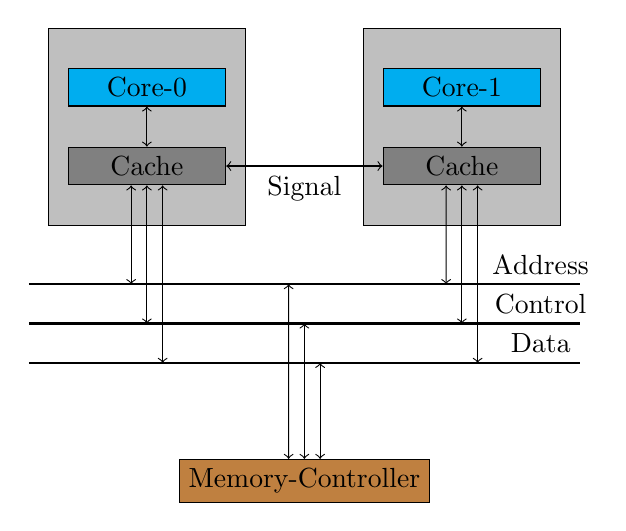
\begin{tikzpicture}
\node (A) at (0,0) [fill=lightgray,draw, minimum size = 2.5cm]{};
\node (A-1) at (0,0.5) [fill=cyan,draw, minimum width = 2cm]{Core-0};

\node (A-2) at (0,-0.5) [fill=gray,draw, minimum width = 2cm]{Cache};

\node (B) at (4,0) [fill=lightgray,draw, minimum size = 2.5cm]{};
\node (B-1) at (4,0.5) [fill=cyan,draw, minimum width = 2cm]{Core-1};

\node (B-2) at (4,-0.5) [fill=gray,draw, minimum width = 2cm]{Cache};


\node (C-1) at (2,-4.5) [fill=brown,draw, minimum width = 2cm]{Memory-Controller};

\draw [<->] (A-2) --node[below]{Signal} (B-2);

\path [thick, draw](-1.5, -2) -- (5.5,-2) ;
\path [thick, draw](-1.5, -2.5) -- (5.5,-2.5);				
\path [thick, draw](-1.5, -3) -- (5.5,-3) ;

\node at (5,-1.75) {Address};
\node at (5,-2.25) {Control};
\node at (5,-2.75) {Data};

\draw [<->] (A-1) -- (A-2);		
\draw [<->] ([xshift=-0.2cm]A-2.south) --(-0.2, -2);
\draw [<->] ([xshift=0.0cm]A-2.south) --(0, -2.5);
\draw [<->] ([xshift=0.2cm]A-2.south) --(0.2, -3);

\draw [<->] (B-1) -- (B-2);		
\draw [<->] ([xshift=-0.2cm]B-2.south) --(3.8, -2);
\draw [<->] ([xshift=0.0cm]B-2.south) --(4, -2.5);
\draw [<->] ([xshift=0.2cm]B-2.south) --(4.2, -3);

%		\draw [<->] (B-1) -- (B-2);		
\draw [<->] (1.8, -2) -- ([xshift=-0.2cm]C-1.north);
\draw [<->] (2, -2.5) -- ([xshift=0.0cm]C-1.north);
\draw [<->] (2.2, -3) -- ([xshift=0.2cm]C-1.north);

\end{tikzpicture}
\end{frame}

\begin{frame}
\frametitle{Vereinfachter Multicore | Read}
\centering
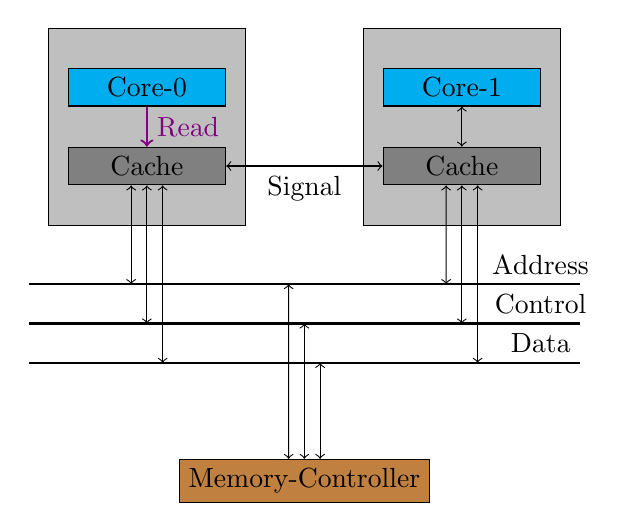
\begin{tikzpicture}
\node (A) at (0,0) [fill=lightgray,draw, minimum size = 2.5cm]{};
\node (A-1) at (0,0.5) [fill=cyan,draw, minimum width = 2cm]{Core-0};

\node (A-2) at (0,-0.5) [fill=gray,draw, minimum width = 2cm]{Cache};

\node (B) at (4,0) [fill=lightgray,draw, minimum size = 2.5cm]{};
\node (B-1) at (4,0.5) [fill=cyan,draw, minimum width = 2cm]{Core-1};

\node (B-2) at (4,-0.5) [fill=gray,draw, minimum width = 2cm]{Cache};


\node (C-1) at (2,-4.5) [fill=brown,draw, minimum width = 2cm]{Memory-Controller};

\draw [<->] (A-2) --node[below]{Signal} (B-2);

\path [thick, draw](-1.5, -2) -- (5.5,-2) ;
\path [thick, draw](-1.5, -2.5) -- (5.5,-2.5);				
\path [thick, draw](-1.5, -3) -- (5.5,-3) ;

\node at (5,-1.75) {Address};
\node at (5,-2.25) {Control};
\node at (5,-2.75) {Data};

\draw [->] [color=violet, thick](A-1) -- node[right	]{Read}(A-2);		
\draw [<->] ([xshift=-0.2cm]A-2.south) --(-0.2, -2);
\draw [<->] ([xshift=0.0cm]A-2.south) --(0, -2.5);
\draw [<->] ([xshift=0.2cm]A-2.south) --(0.2, -3);

\draw [<->] (B-1) -- (B-2);		
\draw [<->] ([xshift=-0.2cm]B-2.south) --(3.8, -2);
\draw [<->] ([xshift=0.0cm]B-2.south) --(4, -2.5);
\draw [<->] ([xshift=0.2cm]B-2.south) --(4.2, -3);

%		\draw [<->] (B-1) -- (B-2);		
\draw [<->] (1.8, -2) -- ([xshift=-0.2cm]C-1.north);
\draw [<->] (2, -2.5) -- ([xshift=0.0cm]C-1.north);
\draw [<->] (2.2, -3) -- ([xshift=0.2cm]C-1.north);

\end{tikzpicture}
\end{frame}

\begin{frame}
\frametitle{Vereinfachter Multicore | Read-Hit}
\centering
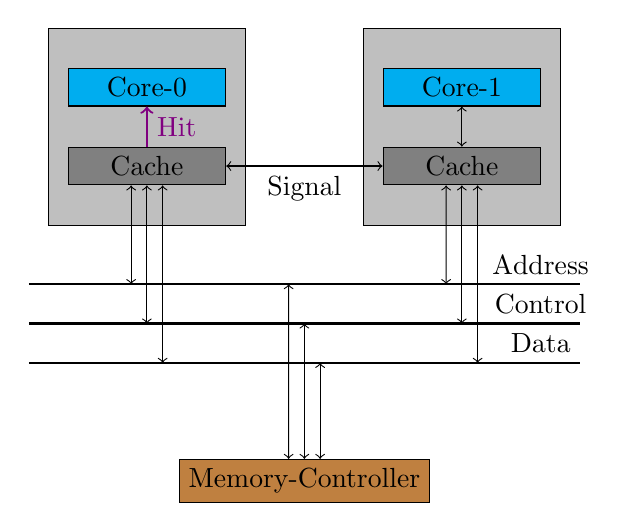
\begin{tikzpicture}
\node (A) at (0,0) [fill=lightgray,draw, minimum size = 2.5cm]{};
\node (A-1) at (0,0.5) [fill=cyan,draw, minimum width = 2cm]{Core-0};

\node (A-2) at (0,-0.5) [fill=gray,draw, minimum width = 2cm]{Cache};

\node (B) at (4,0) [fill=lightgray,draw, minimum size = 2.5cm]{};
\node (B-1) at (4,0.5) [fill=cyan,draw, minimum width = 2cm]{Core-1};

\node (B-2) at (4,-0.5) [fill=gray,draw, minimum width = 2cm]{Cache};


\node (C-1) at (2,-4.5) [fill=brown,draw, minimum width = 2cm]{Memory-Controller};

\draw [<->] (A-2) --node[below]{Signal} (B-2);

\path [thick, draw](-1.5, -2) -- (5.5,-2) ;
\path [thick, draw](-1.5, -2.5) -- (5.5,-2.5);				
\path [thick, draw](-1.5, -3) -- (5.5,-3) ;

\node at (5,-1.75) {Address};
\node at (5,-2.25) {Control};
\node at (5,-2.75) {Data};

\draw [<-] [color=violet, thick](A-1) -- node[right	]{Hit}(A-2);		
\draw [<->] ([xshift=-0.2cm]A-2.south) --(-0.2, -2);
\draw [<->] ([xshift=0.0cm]A-2.south) --(0, -2.5);
\draw [<->] ([xshift=0.2cm]A-2.south) --(0.2, -3);

\draw [<->] (B-1) -- (B-2);		
\draw [<->] ([xshift=-0.2cm]B-2.south) --(3.8, -2);
\draw [<->] ([xshift=0.0cm]B-2.south) --(4, -2.5);
\draw [<->] ([xshift=0.2cm]B-2.south) --(4.2, -3);

%		\draw [<->] (B-1) -- (B-2);		
\draw [<->] (1.8, -2) -- ([xshift=-0.2cm]C-1.north);
\draw [<->] (2, -2.5) -- ([xshift=0.0cm]C-1.north);
\draw [<->] (2.2, -3) -- ([xshift=0.2cm]C-1.north);

\end{tikzpicture}
\end{frame}

\begin{frame}
\frametitle{Vereinfachter Multicore | Read Miss (I/I $\rightarrow$ E/I)}
\centering
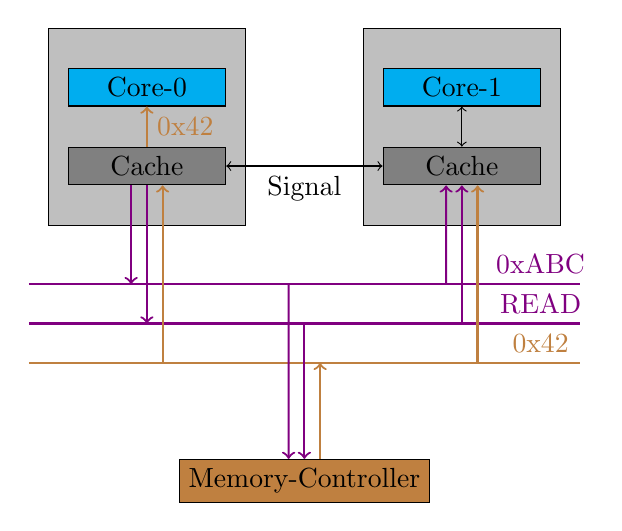
\begin{tikzpicture}
\node (A) at (0,0) [fill=lightgray,draw, minimum size = 2.5cm]{};
\node (A-1) at (0,0.5) [fill=cyan,draw, minimum width = 2cm]{Core-0};

\node (A-2) at (0,-0.5) [fill=gray,draw, minimum width = 2cm]{Cache};

\node (B) at (4,0) [fill=lightgray,draw, minimum size = 2.5cm]{};
\node (B-1) at (4,0.5) [fill=cyan,draw, minimum width = 2cm]{Core-1};

\node (B-2) at (4,-0.5) [fill=gray,draw, minimum width = 2cm]{Cache};


\node (C-1) at (2,-4.5) [fill=brown,draw, minimum width = 2cm]{Memory-Controller};

\draw [<->] (A-2) --node[below]{Signal} (B-2);

\path [color=violet, thick, draw](-1.5, -2) -- (5.5,-2) ;
\path [color=violet, thick, draw](-1.5, -2.5) -- (5.5,-2.5);				
\path [color=brown, thick, draw](-1.5, -3) -- (5.5,-3) ;

\node at (5,-1.75) [color=violet, thick]{0xABC};
\node at (5,-2.25) [color=violet, thick]{READ};
\node at (5,-2.75) [color=brown]{0x42};

\draw [<-] [color=brown, thick](A-1) -- node[right]{0x42}(A-2);		
\draw [->] [color=violet, thick]([xshift=-0.2cm]A-2.south) --(-0.2, -2);
\draw [->] [color=violet, thick]([xshift=0.0cm]A-2.south) --(0, -2.5);
\draw [<-] [color=brown, thick]([xshift=0.2cm]A-2.south) --(0.2, -3);

\draw [<->] (B-1) -- (B-2);		
\draw [<-] [color=violet, thick]([xshift=-0.2cm]B-2.south) --(3.8, -2);
\draw [<-] [color=violet, thick]([xshift=0.0cm]B-2.south) --(4, -2.5);
\draw [<-] [color=brown, thick]([xshift=0.2cm]B-2.south) --(4.2, -3);

%		\draw [<->] (B-1) -- (B-2);		
\draw [->] [color=violet, thick](1.8, -2) -- ([xshift=-0.2cm]C-1.north);
\draw [->] [color=violet, thick](2, -2.5) -- ([xshift=0.0cm]C-1.north);
\draw [<-] [color=brown, thick](2.2, -3) -- ([xshift=0.2cm]C-1.north);

\end{tikzpicture}
\end{frame}

\begin{frame}
\frametitle{Vereinfachter Multicore | Read Miss (I/E $\rightarrow$ S/S)}
\centering
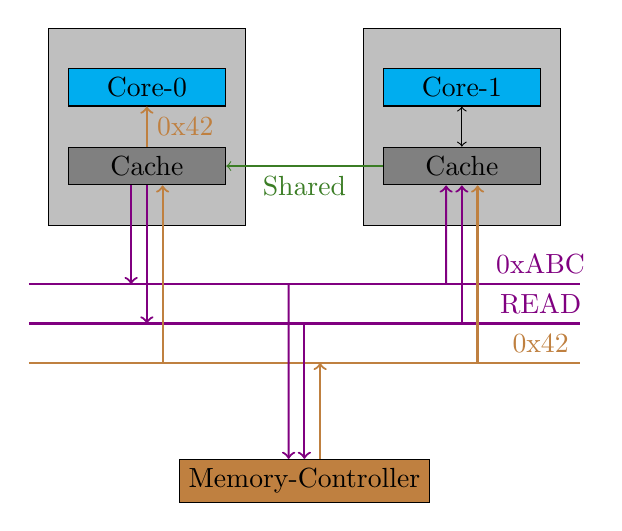
\begin{tikzpicture}
\node (A) at (0,0) [fill=lightgray,draw, minimum size = 2.5cm]{};
\node (A-1) at (0,0.5) [fill=cyan,draw, minimum width = 2cm]{Core-0};

\node (A-2) at (0,-0.5) [fill=gray,draw, minimum width = 2cm]{Cache};

\node (B) at (4,0) [fill=lightgray,draw, minimum size = 2.5cm]{};
\node (B-1) at (4,0.5) [fill=cyan,draw, minimum width = 2cm]{Core-1};

\node (B-2) at (4,-0.5) [fill=gray,draw, minimum width = 2cm]{Cache};


\node (C-1) at (2,-4.5) [fill=brown,draw, minimum width = 2cm]{Memory-Controller};

\draw [<-] [color=OliveGreen](A-2) --node[below]{Shared} (B-2);

\path [color=violet, thick, draw](-1.5, -2) -- (5.5,-2) ;
\path [color=violet, thick, draw](-1.5, -2.5) -- (5.5,-2.5);				
\path [color=brown, thick, draw](-1.5, -3) -- (5.5,-3) ;

\node at (5,-1.75) [color=violet, thick]{0xABC};
\node at (5,-2.25) [color=violet, thick]{READ};
\node at (5,-2.75) [color=brown]{0x42};

\draw [<-] [color=brown, thick](A-1) -- node[right]{0x42}(A-2);		
\draw [->] [color=violet, thick]([xshift=-0.2cm]A-2.south) --(-0.2, -2);
\draw [->] [color=violet, thick]([xshift=0.0cm]A-2.south) --(0, -2.5);
\draw [<-] [color=brown, thick]([xshift=0.2cm]A-2.south) --(0.2, -3);

\draw [<->] (B-1) -- (B-2);		
\draw [<-] [color=violet, thick]([xshift=-0.2cm]B-2.south) --(3.8, -2);
\draw [<-] [color=violet, thick]([xshift=0.0cm]B-2.south) --(4, -2.5);
\draw [<-] [color=brown, thick]([xshift=0.2cm]B-2.south) --(4.2, -3);

%		\draw [<->] (B-1) -- (B-2);		
\draw [->] [color=violet, thick](1.8, -2) -- ([xshift=-0.2cm]C-1.north);
\draw [->] [color=violet, thick](2, -2.5) -- ([xshift=0.0cm]C-1.north);
\draw [<-] [color=brown, thick](2.2, -3) -- ([xshift=0.2cm]C-1.north);

\end{tikzpicture}
\end{frame}

\begin{frame}
\frametitle{Vereinfachter Multicore | Read Miss (I/S $\rightarrow$ S/S)}
\centering
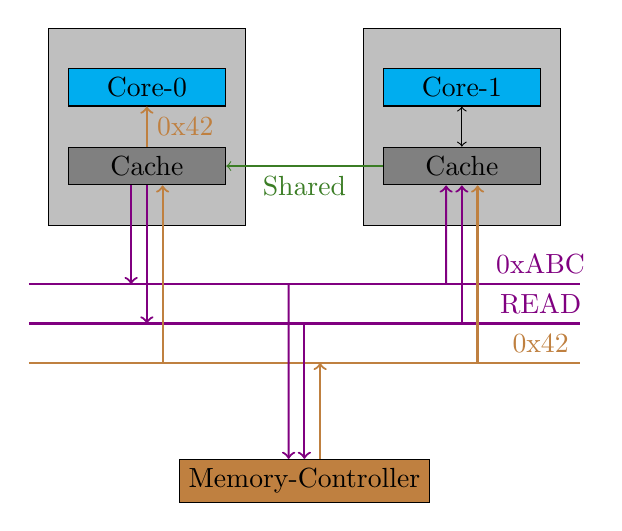
\begin{tikzpicture}
\node (A) at (0,0) [fill=lightgray,draw, minimum size = 2.5cm]{};
\node (A-1) at (0,0.5) [fill=cyan,draw, minimum width = 2cm]{Core-0};

\node (A-2) at (0,-0.5) [fill=gray,draw, minimum width = 2cm]{Cache};

\node (B) at (4,0) [fill=lightgray,draw, minimum size = 2.5cm]{};
\node (B-1) at (4,0.5) [fill=cyan,draw, minimum width = 2cm]{Core-1};

\node (B-2) at (4,-0.5) [fill=gray,draw, minimum width = 2cm]{Cache};


\node (C-1) at (2,-4.5) [fill=brown,draw, minimum width = 2cm]{Memory-Controller};

\draw [<-] [color=OliveGreen](A-2) --node[below]{Shared} (B-2);

\path [color=violet, thick, draw](-1.5, -2) -- (5.5,-2) ;
\path [color=violet, thick, draw](-1.5, -2.5) -- (5.5,-2.5);				
\path [color=brown, thick, draw](-1.5, -3) -- (5.5,-3) ;

\node at (5,-1.75) [color=violet, thick]{0xABC};
\node at (5,-2.25) [color=violet, thick]{READ};
\node at (5,-2.75) [color=brown]{0x42};

\draw [<-] [color=brown, thick](A-1) -- node[right]{0x42}(A-2);		
\draw [->] [color=violet, thick]([xshift=-0.2cm]A-2.south) --(-0.2, -2);
\draw [->] [color=violet, thick]([xshift=0.0cm]A-2.south) --(0, -2.5);
\draw [<-] [color=brown, thick]([xshift=0.2cm]A-2.south) --(0.2, -3);

\draw [<->] (B-1) -- (B-2);		
\draw [<-] [color=violet, thick]([xshift=-0.2cm]B-2.south) --(3.8, -2);
\draw [<-] [color=violet, thick]([xshift=0.0cm]B-2.south) --(4, -2.5);
\draw [<-] [color=brown, thick]([xshift=0.2cm]B-2.south) --(4.2, -3);

%		\draw [<->] (B-1) -- (B-2);		
\draw [->] [color=violet, thick](1.8, -2) -- ([xshift=-0.2cm]C-1.north);
\draw [->] [color=violet, thick](2, -2.5) -- ([xshift=0.0cm]C-1.north);
\draw [<-] [color=brown, thick](2.2, -3) -- ([xshift=0.2cm]C-1.north);

\end{tikzpicture}
\end{frame}

\begin{frame}
\frametitle{Vereinfachter Multicore | Read Miss (I/M $\rightarrow$ S/S)}
\centering
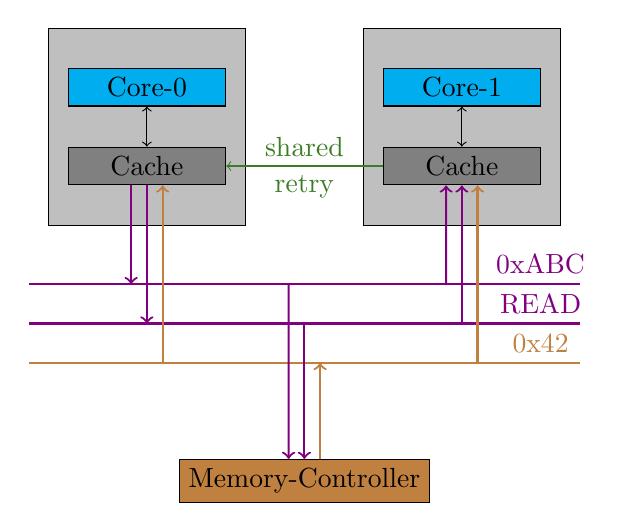
\begin{tikzpicture}
\node (A) at (0,0) [fill=lightgray,draw, minimum size = 2.5cm]{};
\node (A-1) at (0,0.5) [fill=cyan,draw, minimum width = 2cm]{Core-0};

\node (A-2) at (0,-0.5) [fill=gray,draw, minimum width = 2cm]{Cache};

\node (B) at (4,0) [fill=lightgray,draw, minimum size = 2.5cm]{};
\node (B-1) at (4,0.5) [fill=cyan,draw, minimum width = 2cm]{Core-1};

\node (B-2) at (4,-0.5) [fill=gray,draw, minimum width = 2cm]{Cache};


\node (C-1) at (2,-4.5) [fill=brown,draw, minimum width = 2cm]{Memory-Controller};

\draw [<-] [color=OliveGreen](A-2) --node[below]{retry}node[above]{shared} (B-2);

\path [color=violet, thick, draw](-1.5, -2) -- (5.5,-2) ;
\path [color=violet, thick, draw](-1.5, -2.5) -- (5.5,-2.5);				
\path [color=brown, thick, draw](-1.5, -3) -- (5.5,-3) ;

\node at (5,-1.75) [color=violet, thick]{0xABC};
\node at (5,-2.25) [color=violet, thick]{READ};
\node at (5,-2.75) [color=brown]{0x42};

\draw [<->] (A-1) -- (A-2);		
\draw [->] [color=violet, thick]([xshift=-0.2cm]A-2.south) --(-0.2, -2);
\draw [->] [color=violet, thick]([xshift=0.0cm]A-2.south) --(0, -2.5);
\draw [<-] [color=brown, thick]([xshift=0.2cm]A-2.south) --(0.2, -3);

\draw [<->] (B-1) -- (B-2);		
\draw [<-] [color=violet, thick]([xshift=-0.2cm]B-2.south) --(3.8, -2);
\draw [<-] [color=violet, thick]([xshift=0.0cm]B-2.south) --(4, -2.5);
\draw [<-] [color=brown, thick]([xshift=0.2cm]B-2.south) --(4.2, -3);

%		\draw [<->] (B-1) -- (B-2);		
\draw [->] [color=violet, thick](1.8, -2) -- ([xshift=-0.2cm]C-1.north);
\draw [->] [color=violet, thick](2, -2.5) -- ([xshift=0.0cm]C-1.north);
\draw [<-] [color=brown, thick](2.2, -3) -- ([xshift=0.2cm]C-1.north);

\end{tikzpicture}
\end{frame}

\begin{frame}
\frametitle{Vereinfachter Multicore | Read Miss (I/M $\rightarrow$ S/S) (2)}
\centering
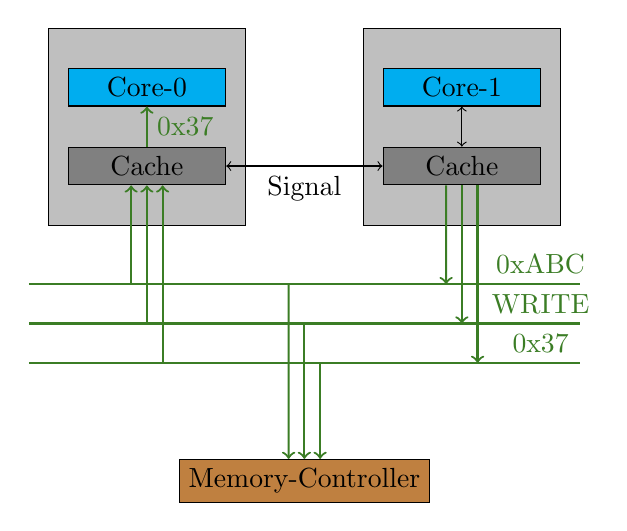
\begin{tikzpicture}
\node (A) at (0,0) [fill=lightgray,draw, minimum size = 2.5cm]{};
\node (A-1) at (0,0.5) [fill=cyan,draw, minimum width = 2cm]{Core-0};

\node (A-2) at (0,-0.5) [fill=gray,draw, minimum width = 2cm]{Cache};

\node (B) at (4,0) [fill=lightgray,draw, minimum size = 2.5cm]{};
\node (B-1) at (4,0.5) [fill=cyan,draw, minimum width = 2cm]{Core-1};

\node (B-2) at (4,-0.5) [fill=gray,draw, minimum width = 2cm]{Cache};


\node (C-1) at (2,-4.5) [fill=brown,draw, minimum width = 2cm]{Memory-Controller};

\draw [<->] (A-2) --node[below]{Signal}(B-2);

\path [color=OliveGreen, thick, draw](-1.5, -2) -- (5.5,-2) ;
\path [color=OliveGreen, thick, draw](-1.5, -2.5) -- (5.5,-2.5);				
\path [color=OliveGreen, thick, draw](-1.5, -3) -- (5.5,-3) ;

\node at (5,-1.75) [color=OliveGreen, thick]{0xABC};
\node at (5,-2.25) [color=OliveGreen, thick]{WRITE};
\node at (5,-2.75) [color=OliveGreen]{0x37};

\draw [<-] [color=OliveGreen, thick] (A-1) -- node[right]{0x37}(A-2);		
\draw [<-] [color=OliveGreen, thick]([xshift=-0.2cm]A-2.south) --(-0.2, -2);
\draw [<-] [color=OliveGreen, thick]([xshift=0.0cm]A-2.south) --(0, -2.5);
\draw [<-] [color=OliveGreen, thick]([xshift=0.2cm]A-2.south) --(0.2, -3);

\draw [<->] (B-1) -- (B-2);		
\draw [->] [color=OliveGreen, thick]([xshift=-0.2cm]B-2.south) --(3.8, -2);
\draw [->] [color=OliveGreen, thick]([xshift=0.0cm]B-2.south) --(4, -2.5);
\draw [->] [color=OliveGreen, thick]([xshift=0.2cm]B-2.south) --(4.2, -3);

%		\draw [<->] (B-1) -- (B-2);		
\draw [->] [color=OliveGreen, thick](1.8, -2) -- ([xshift=-0.2cm]C-1.north);
\draw [->] [color=OliveGreen, thick](2, -2.5) -- ([xshift=0.0cm]C-1.north);
\draw [->] [color=OliveGreen, thick](2.2, -3) -- ([xshift=0.2cm]C-1.north);

\end{tikzpicture}
\end{frame}

\begin{frame}
\frametitle{Vereinfachter Multicore | Write}
\centering
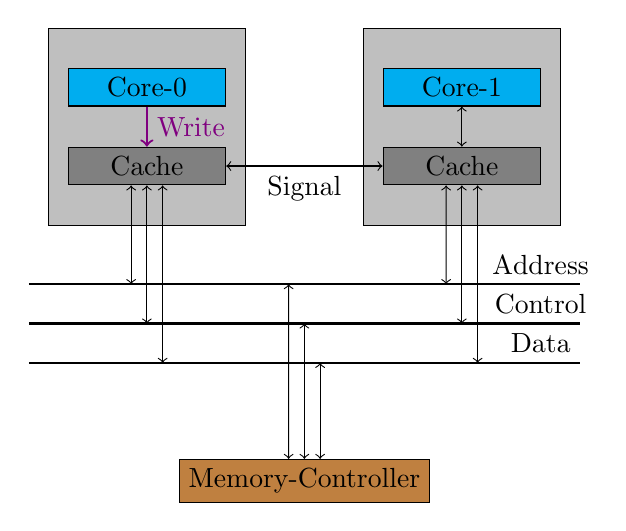
\begin{tikzpicture}
\node (A) at (0,0) [fill=lightgray,draw, minimum size = 2.5cm]{};
\node (A-1) at (0,0.5) [fill=cyan,draw, minimum width = 2cm]{Core-0};

\node (A-2) at (0,-0.5) [fill=gray,draw, minimum width = 2cm]{Cache};

\node (B) at (4,0) [fill=lightgray,draw, minimum size = 2.5cm]{};
\node (B-1) at (4,0.5) [fill=cyan,draw, minimum width = 2cm]{Core-1};

\node (B-2) at (4,-0.5) [fill=gray,draw, minimum width = 2cm]{Cache};


\node (C-1) at (2,-4.5) [fill=brown,draw, minimum width = 2cm]{Memory-Controller};

\draw [<->] (A-2) --node[below]{Signal} (B-2);

\path [thick, draw](-1.5, -2) -- (5.5,-2) ;
\path [thick, draw](-1.5, -2.5) -- (5.5,-2.5);				
\path [thick, draw](-1.5, -3) -- (5.5,-3) ;

\node at (5,-1.75) {Address};
\node at (5,-2.25) {Control};
\node at (5,-2.75) {Data};

\draw [->] [color=violet, thick](A-1) -- node[right	]{Write}(A-2);		
\draw [<->] ([xshift=-0.2cm]A-2.south) --(-0.2, -2);
\draw [<->] ([xshift=0.0cm]A-2.south) --(0, -2.5);
\draw [<->] ([xshift=0.2cm]A-2.south) --(0.2, -3);

\draw [<->] (B-1) -- (B-2);		
\draw [<->] ([xshift=-0.2cm]B-2.south) --(3.8, -2);
\draw [<->] ([xshift=0.0cm]B-2.south) --(4, -2.5);
\draw [<->] ([xshift=0.2cm]B-2.south) --(4.2, -3);

%		\draw [<->] (B-1) -- (B-2);		
\draw [<->] (1.8, -2) -- ([xshift=-0.2cm]C-1.north);
\draw [<->] (2, -2.5) -- ([xshift=0.0cm]C-1.north);
\draw [<->] (2.2, -3) -- ([xshift=0.2cm]C-1.north);

\end{tikzpicture}
\end{frame}

\begin{frame}
\frametitle{Vereinfachter Multicore | Write Hit (M/I $\rightarrow$ M/I)}
\centering
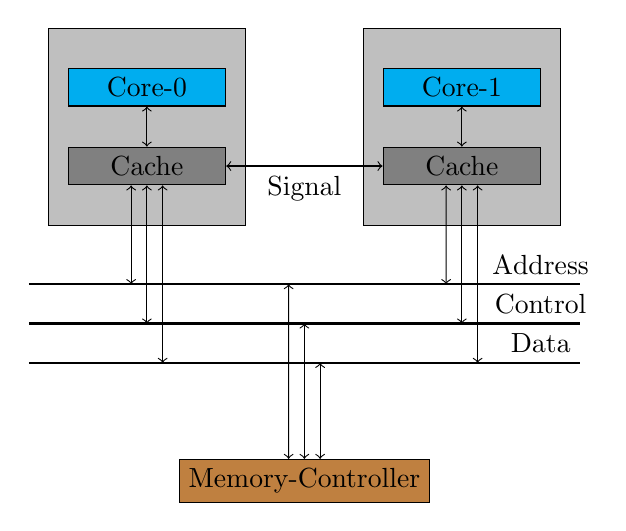
\begin{tikzpicture}
\node (A) at (0,0) [fill=lightgray,draw, minimum size = 2.5cm]{};
\node (A-1) at (0,0.5) [fill=cyan,draw, minimum width = 2cm]{Core-0};

\node (A-2) at (0,-0.5) [fill=gray,draw, minimum width = 2cm]{Cache};

\node (B) at (4,0) [fill=lightgray,draw, minimum size = 2.5cm]{};
\node (B-1) at (4,0.5) [fill=cyan,draw, minimum width = 2cm]{Core-1};

\node (B-2) at (4,-0.5) [fill=gray,draw, minimum width = 2cm]{Cache};


\node (C-1) at (2,-4.5) [fill=brown,draw, minimum width = 2cm]{Memory-Controller};

\draw [<->] (A-2) --node[below]{Signal} (B-2);

\path [thick, draw](-1.5, -2) -- (5.5,-2) ;
\path [thick, draw](-1.5, -2.5) -- (5.5,-2.5);				
\path [thick, draw](-1.5, -3) -- (5.5,-3) ;

\node at (5,-1.75) {Address};
\node at (5,-2.25) {Control};
\node at (5,-2.75) {Data};

\draw [<->] (A-1) -- (A-2);		
\draw [<->] ([xshift=-0.2cm]A-2.south) --(-0.2, -2);
\draw [<->] ([xshift=0.0cm]A-2.south) --(0, -2.5);
\draw [<->] ([xshift=0.2cm]A-2.south) --(0.2, -3);

\draw [<->] (B-1) -- (B-2);		
\draw [<->] ([xshift=-0.2cm]B-2.south) --(3.8, -2);
\draw [<->] ([xshift=0.0cm]B-2.south) --(4, -2.5);
\draw [<->] ([xshift=0.2cm]B-2.south) --(4.2, -3);

%		\draw [<->] (B-1) -- (B-2);		
\draw [<->] (1.8, -2) -- ([xshift=-0.2cm]C-1.north);
\draw [<->] (2, -2.5) -- ([xshift=0.0cm]C-1.north);
\draw [<->] (2.2, -3) -- ([xshift=0.2cm]C-1.north);

\end{tikzpicture}
\end{frame}

\begin{frame}
\frametitle{Vereinfachter Multicore | Write Hit (E/I $\rightarrow$ M/I)}
\centering
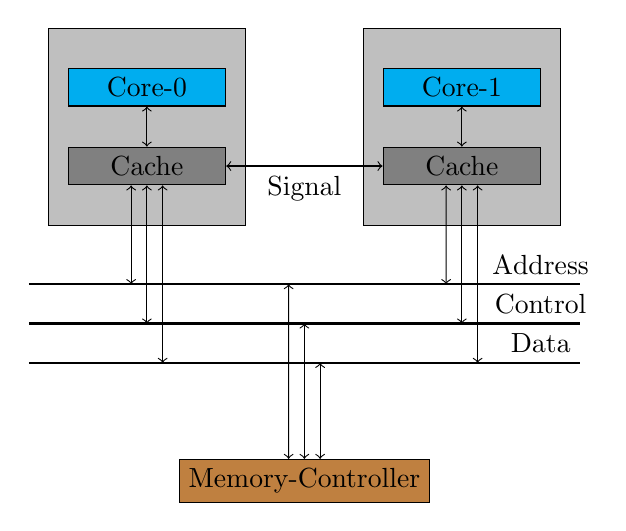
\begin{tikzpicture}
\node (A) at (0,0) [fill=lightgray,draw, minimum size = 2.5cm]{};
\node (A-1) at (0,0.5) [fill=cyan,draw, minimum width = 2cm]{Core-0};

\node (A-2) at (0,-0.5) [fill=gray,draw, minimum width = 2cm]{Cache};

\node (B) at (4,0) [fill=lightgray,draw, minimum size = 2.5cm]{};
\node (B-1) at (4,0.5) [fill=cyan,draw, minimum width = 2cm]{Core-1};

\node (B-2) at (4,-0.5) [fill=gray,draw, minimum width = 2cm]{Cache};


\node (C-1) at (2,-4.5) [fill=brown,draw, minimum width = 2cm]{Memory-Controller};

\draw [<->] (A-2) --node[below]{Signal} (B-2);

\path [thick, draw](-1.5, -2) -- (5.5,-2) ;
\path [thick, draw](-1.5, -2.5) -- (5.5,-2.5);				
\path [thick, draw](-1.5, -3) -- (5.5,-3) ;

\node at (5,-1.75) {Address};
\node at (5,-2.25) {Control};
\node at (5,-2.75) {Data};

\draw [<->] (A-1) -- (A-2);		
\draw [<->] ([xshift=-0.2cm]A-2.south) --(-0.2, -2);
\draw [<->] ([xshift=0.0cm]A-2.south) --(0, -2.5);
\draw [<->] ([xshift=0.2cm]A-2.south) --(0.2, -3);

\draw [<->] (B-1) -- (B-2);		
\draw [<->] ([xshift=-0.2cm]B-2.south) --(3.8, -2);
\draw [<->] ([xshift=0.0cm]B-2.south) --(4, -2.5);
\draw [<->] ([xshift=0.2cm]B-2.south) --(4.2, -3);

%		\draw [<->] (B-1) -- (B-2);		
\draw [<->] (1.8, -2) -- ([xshift=-0.2cm]C-1.north);
\draw [<->] (2, -2.5) -- ([xshift=0.0cm]C-1.north);
\draw [<->] (2.2, -3) -- ([xshift=0.2cm]C-1.north);

\end{tikzpicture}
\end{frame}


\begin{frame}
\frametitle{Vereinfachter Multicore | Write Hit (S/S $\rightarrow$ M/I)}
\centering
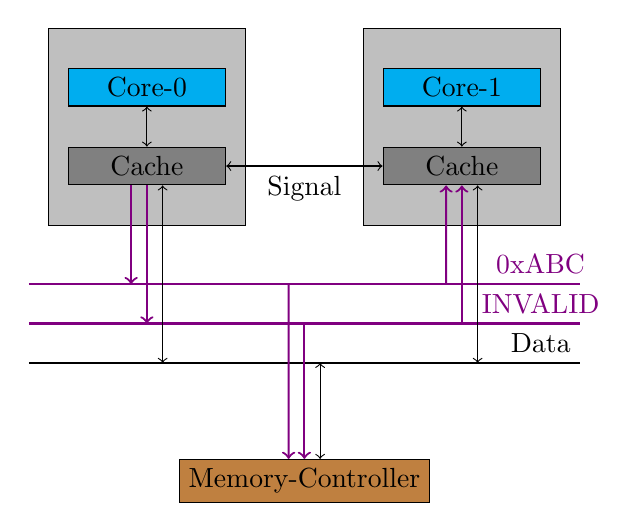
\begin{tikzpicture}
\node (A) at (0,0) [fill=lightgray,draw, minimum size = 2.5cm]{};
\node (A-1) at (0,0.5) [fill=cyan,draw, minimum width = 2cm]{Core-0};

\node (A-2) at (0,-0.5) [fill=gray,draw, minimum width = 2cm]{Cache};

\node (B) at (4,0) [fill=lightgray,draw, minimum size = 2.5cm]{};
\node (B-1) at (4,0.5) [fill=cyan,draw, minimum width = 2cm]{Core-1};

\node (B-2) at (4,-0.5) [fill=gray,draw, minimum width = 2cm]{Cache};


\node (C-1) at (2,-4.5) [fill=brown,draw, minimum width = 2cm]{Memory-Controller};

\draw [<->] (A-2) --node[below]{Signal} (B-2);

\path [color=violet, thick, draw](-1.5, -2) -- (5.5,-2) ;
\path [color=violet, thick, draw](-1.5, -2.5) -- (5.5,-2.5);				
\path [thick, draw](-1.5, -3) -- (5.5,-3) ;

\node at (5,-1.75) [color=violet, thick]{0xABC};
\node at (5,-2.25) [color=violet, thick]{INVALID};
\node at (5,-2.75) {Data};

\draw [<->] (A-1) -- (A-2);		
\draw [->] [color=violet, thick]([xshift=-0.2cm]A-2.south) --(-0.2, -2);
\draw [->] [color=violet, thick]([xshift=0.0cm]A-2.south) --(0, -2.5);
\draw [<->] ([xshift=0.2cm]A-2.south) --(0.2, -3);

\draw [<->] (B-1) -- (B-2);		
\draw [<-] [color=violet, thick]([xshift=-0.2cm]B-2.south) --(3.8, -2);
\draw [<-] [color=violet, thick]([xshift=0.0cm]B-2.south) --(4, -2.5);
\draw [<->] ([xshift=0.2cm]B-2.south) --(4.2, -3);

%		\draw [<->] (B-1) -- (B-2);		
\draw [->] [color=violet, thick](1.8, -2) -- ([xshift=-0.2cm]C-1.north);
\draw [->] [color=violet, thick](2, -2.5) -- ([xshift=0.0cm]C-1.north);
\draw [<->] (2.2, -3) -- ([xshift=0.2cm]C-1.north);

\end{tikzpicture}
\end{frame}

\begin{frame}
\frametitle{Vereinfachter Multicore | Write Miss (I/E $\rightarrow$ M/I)}
\centering
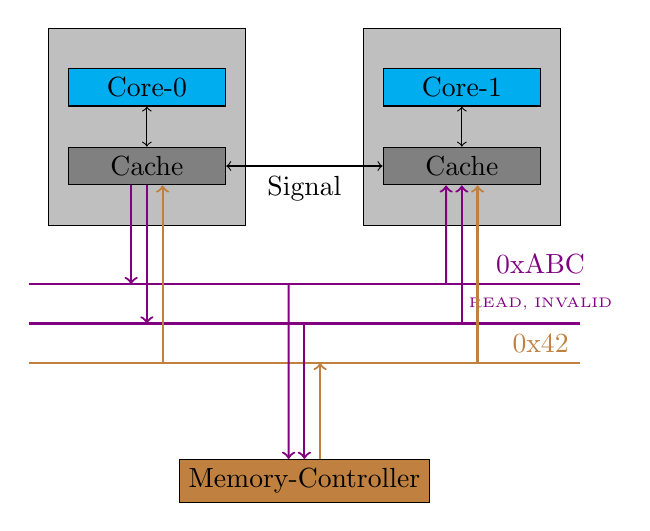
\begin{tikzpicture}
\node (A) at (0,0) [fill=lightgray,draw, minimum size = 2.5cm]{};
\node (A-1) at (0,0.5) [fill=cyan,draw, minimum width = 2cm]{Core-0};

\node (A-2) at (0,-0.5) [fill=gray,draw, minimum width = 2cm]{Cache};

\node (B) at (4,0) [fill=lightgray,draw, minimum size = 2.5cm]{};
\node (B-1) at (4,0.5) [fill=cyan,draw, minimum width = 2cm]{Core-1};

\node (B-2) at (4,-0.5) [fill=gray,draw, minimum width = 2cm]{Cache};


\node (C-1) at (2,-4.5) [fill=brown,draw, minimum width = 2cm]{Memory-Controller};

\draw [<->] (A-2) --node[below]{Signal} (B-2);

\path [color=violet, thick, draw](-1.5, -2) -- (5.5,-2) ;
\path [color=violet, thick, draw](-1.5, -2.5) -- (5.5,-2.5);				
\path [color=brown, thick, draw](-1.5, -3) -- (5.5,-3) ;

\node at (5,-1.75) [color=violet, thick]{0xABC};
\node at (5,-2.25) [color=violet, thick]{\tiny READ, INVALID};
\node at (5,-2.75) [color=brown]{0x42};

\draw [<->] (A-1) -- (A-2);		
\draw [->] [color=violet, thick]([xshift=-0.2cm]A-2.south) --(-0.2, -2);
\draw [->] [color=violet, thick]([xshift=0.0cm]A-2.south) --(0, -2.5);
\draw [<-] [color=brown, thick]([xshift=0.2cm]A-2.south) --(0.2, -3);

\draw [<->] (B-1) -- (B-2);		
\draw [<-] [color=violet, thick]([xshift=-0.2cm]B-2.south) --(3.8, -2);
\draw [<-] [color=violet, thick]([xshift=0.0cm]B-2.south) --(4, -2.5);
\draw [<-] [color=brown, thick]([xshift=0.2cm]B-2.south) --(4.2, -3);

%		\draw [<->] (B-1) -- (B-2);		
\draw [->] [color=violet, thick](1.8, -2) -- ([xshift=-0.2cm]C-1.north);
\draw [->] [color=violet, thick](2, -2.5) -- ([xshift=0.0cm]C-1.north);
\draw [<-] [color=brown, thick](2.2, -3) -- ([xshift=0.2cm]C-1.north);

\end{tikzpicture}
\end{frame}

\begin{frame}
\frametitle{Vereinfachter Multicore | Write Miss (I/S $\rightarrow$ M/I)}
\centering
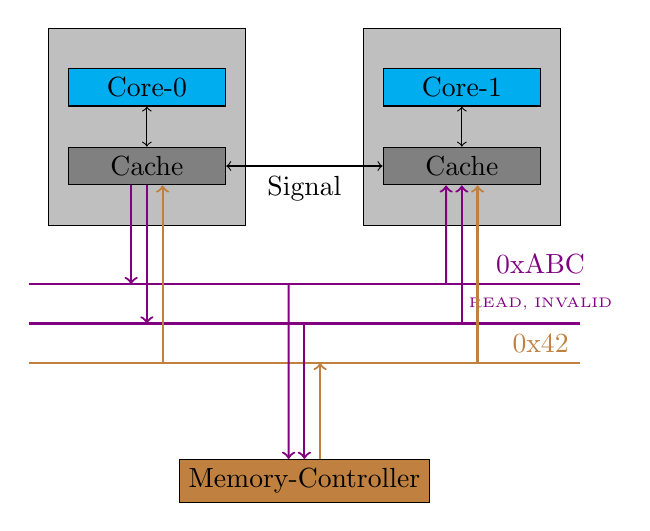
\begin{tikzpicture}
\node (A) at (0,0) [fill=lightgray,draw, minimum size = 2.5cm]{};
\node (A-1) at (0,0.5) [fill=cyan,draw, minimum width = 2cm]{Core-0};

\node (A-2) at (0,-0.5) [fill=gray,draw, minimum width = 2cm]{Cache};

\node (B) at (4,0) [fill=lightgray,draw, minimum size = 2.5cm]{};
\node (B-1) at (4,0.5) [fill=cyan,draw, minimum width = 2cm]{Core-1};

\node (B-2) at (4,-0.5) [fill=gray,draw, minimum width = 2cm]{Cache};


\node (C-1) at (2,-4.5) [fill=brown,draw, minimum width = 2cm]{Memory-Controller};

\draw [<->] (A-2) --node[below]{Signal} (B-2);

\path [color=violet, thick, draw](-1.5, -2) -- (5.5,-2) ;
\path [color=violet, thick, draw](-1.5, -2.5) -- (5.5,-2.5);				
\path [color=brown, thick, draw](-1.5, -3) -- (5.5,-3) ;

\node at (5,-1.75) [color=violet, thick]{0xABC};
\node at (5,-2.25) [color=violet, thick]{\tiny READ, INVALID};
\node at (5,-2.75) [color=brown]{0x42};

\draw [<->] (A-1) -- (A-2);		
\draw [->] [color=violet, thick]([xshift=-0.2cm]A-2.south) --(-0.2, -2);
\draw [->] [color=violet, thick]([xshift=0.0cm]A-2.south) --(0, -2.5);
\draw [<-] [color=brown, thick]([xshift=0.2cm]A-2.south) --(0.2, -3);

\draw [<->] (B-1) -- (B-2);		
\draw [<-] [color=violet, thick]([xshift=-0.2cm]B-2.south) --(3.8, -2);
\draw [<-] [color=violet, thick]([xshift=0.0cm]B-2.south) --(4, -2.5);
\draw [<-] [color=brown, thick]([xshift=0.2cm]B-2.south) --(4.2, -3);

%		\draw [<->] (B-1) -- (B-2);		
\draw [->] [color=violet, thick](1.8, -2) -- ([xshift=-0.2cm]C-1.north);
\draw [->] [color=violet, thick](2, -2.5) -- ([xshift=0.0cm]C-1.north);
\draw [<-] [color=brown, thick](2.2, -3) -- ([xshift=0.2cm]C-1.north);

\end{tikzpicture}
\end{frame}

\begin{frame}
\frametitle{Vereinfachter Multicore | Write Miss (I/I $\rightarrow$ M/I)}
\centering
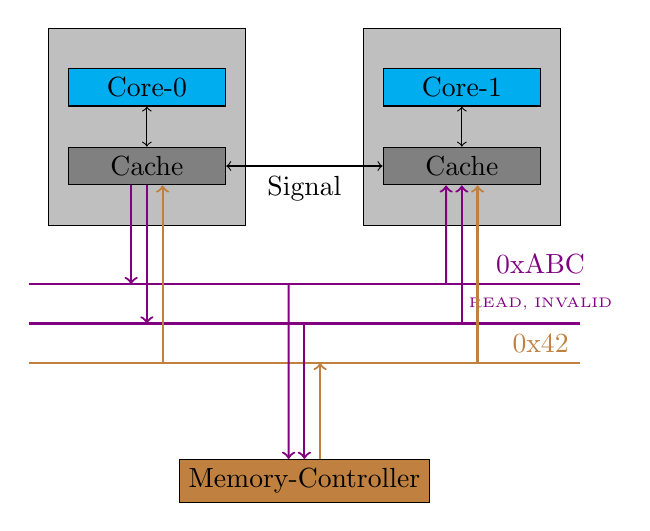
\begin{tikzpicture}
\node (A) at (0,0) [fill=lightgray,draw, minimum size = 2.5cm]{};
\node (A-1) at (0,0.5) [fill=cyan,draw, minimum width = 2cm]{Core-0};

\node (A-2) at (0,-0.5) [fill=gray,draw, minimum width = 2cm]{Cache};

\node (B) at (4,0) [fill=lightgray,draw, minimum size = 2.5cm]{};
\node (B-1) at (4,0.5) [fill=cyan,draw, minimum width = 2cm]{Core-1};

\node (B-2) at (4,-0.5) [fill=gray,draw, minimum width = 2cm]{Cache};


\node (C-1) at (2,-4.5) [fill=brown,draw, minimum width = 2cm]{Memory-Controller};

\draw [<->] (A-2) --node[below]{Signal} (B-2);

\path [color=violet, thick, draw](-1.5, -2) -- (5.5,-2) ;
\path [color=violet, thick, draw](-1.5, -2.5) -- (5.5,-2.5);				
\path [color=brown, thick, draw](-1.5, -3) -- (5.5,-3) ;

\node at (5,-1.75) [color=violet, thick]{0xABC};
\node at (5,-2.25) [color=violet, thick]{\tiny READ, INVALID};
\node at (5,-2.75) [color=brown]{0x42};

\draw [<->] (A-1) -- (A-2);		
\draw [->] [color=violet, thick]([xshift=-0.2cm]A-2.south) --(-0.2, -2);
\draw [->] [color=violet, thick]([xshift=0.0cm]A-2.south) --(0, -2.5);
\draw [<-] [color=brown, thick]([xshift=0.2cm]A-2.south) --(0.2, -3);

\draw [<->] (B-1) -- (B-2);		
\draw [<-] [color=violet, thick]([xshift=-0.2cm]B-2.south) --(3.8, -2);
\draw [<-] [color=violet, thick]([xshift=0.0cm]B-2.south) --(4, -2.5);
\draw [<-] [color=brown, thick]([xshift=0.2cm]B-2.south) --(4.2, -3);

%		\draw [<->] (B-1) -- (B-2);		
\draw [->] [color=violet, thick](1.8, -2) -- ([xshift=-0.2cm]C-1.north);
\draw [->] [color=violet, thick](2, -2.5) -- ([xshift=0.0cm]C-1.north);
\draw [<-] [color=brown, thick](2.2, -3) -- ([xshift=0.2cm]C-1.north);

\end{tikzpicture}
\end{frame}

\begin{frame}
\frametitle{Vereinfachter Multicore | Write Miss (I/M $\rightarrow$ M/I)}
\centering
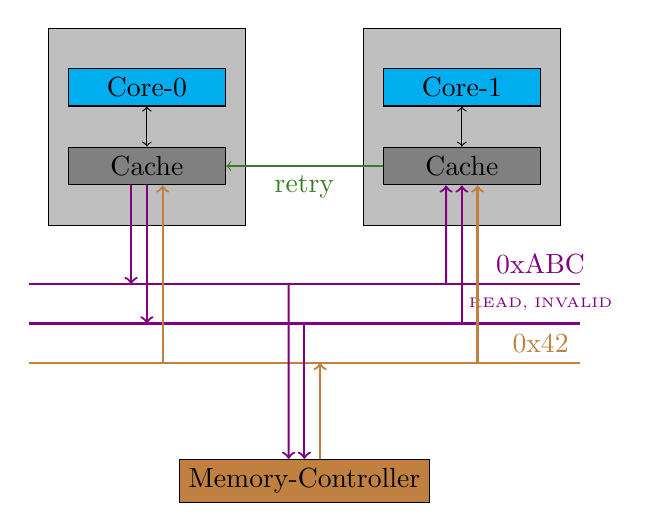
\begin{tikzpicture}
\node (A) at (0,0) [fill=lightgray,draw, minimum size = 2.5cm]{};
\node (A-1) at (0,0.5) [fill=cyan,draw, minimum width = 2cm]{Core-0};

\node (A-2) at (0,-0.5) [fill=gray,draw, minimum width = 2cm]{Cache};

\node (B) at (4,0) [fill=lightgray,draw, minimum size = 2.5cm]{};
\node (B-1) at (4,0.5) [fill=cyan,draw, minimum width = 2cm]{Core-1};

\node (B-2) at (4,-0.5) [fill=gray,draw, minimum width = 2cm]{Cache};


\node (C-1) at (2,-4.5) [fill=brown,draw, minimum width = 2cm]{Memory-Controller};

\draw [<-] [color=OliveGreen](A-2) --node[below]{retry} (B-2);

\path [color=violet, thick, draw](-1.5, -2) -- (5.5,-2) ;
\path [color=violet, thick, draw](-1.5, -2.5) -- (5.5,-2.5);				
\path [color=brown, thick, draw](-1.5, -3) -- (5.5,-3) ;

\node at (5,-1.75) [color=violet, thick]{0xABC};
\node at (5,-2.25) [color=violet, thick]{\tiny READ, INVALID};
\node at (5,-2.75) [color=brown]{0x42};

\draw [<->] (A-1) -- (A-2);		
\draw [->] [color=violet, thick]([xshift=-0.2cm]A-2.south) --(-0.2, -2);
\draw [->] [color=violet, thick]([xshift=0.0cm]A-2.south) --(0, -2.5);
\draw [<-] [color=brown, thick]([xshift=0.2cm]A-2.south) --(0.2, -3);

\draw [<->] (B-1) -- (B-2);		
\draw [<-] [color=violet, thick]([xshift=-0.2cm]B-2.south) --(3.8, -2);
\draw [<-] [color=violet, thick]([xshift=0.0cm]B-2.south) --(4, -2.5);
\draw [<-] [color=brown, thick]([xshift=0.2cm]B-2.south) --(4.2, -3);

%		\draw [<->] (B-1) -- (B-2);		
\draw [->] [color=violet, thick](1.8, -2) -- ([xshift=-0.2cm]C-1.north);
\draw [->] [color=violet, thick](2, -2.5) -- ([xshift=0.0cm]C-1.north);
\draw [<-] [color=brown, thick](2.2, -3) -- ([xshift=0.2cm]C-1.north);

\end{tikzpicture}
\end{frame}

\begin{frame}
\frametitle{Vereinfachter Multicore | Write Miss (I/M $\rightarrow$ M/I) (2)}
\centering
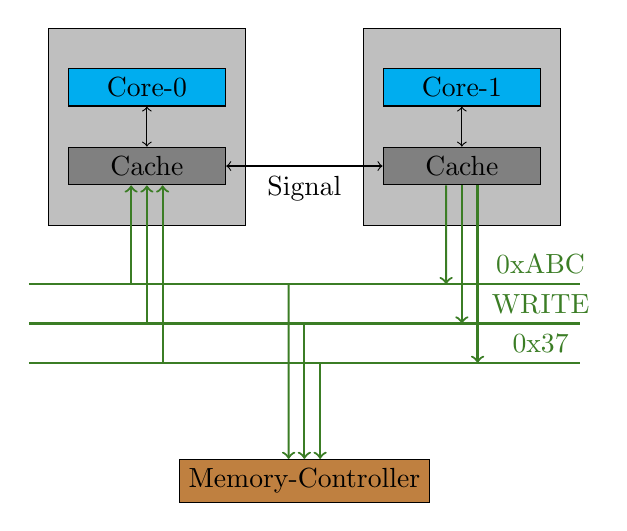
\begin{tikzpicture}
\node (A) at (0,0) [fill=lightgray,draw, minimum size = 2.5cm]{};
\node (A-1) at (0,0.5) [fill=cyan,draw, minimum width = 2cm]{Core-0};

\node (A-2) at (0,-0.5) [fill=gray,draw, minimum width = 2cm]{Cache};

\node (B) at (4,0) [fill=lightgray,draw, minimum size = 2.5cm]{};
\node (B-1) at (4,0.5) [fill=cyan,draw, minimum width = 2cm]{Core-1};

\node (B-2) at (4,-0.5) [fill=gray,draw, minimum width = 2cm]{Cache};


\node (C-1) at (2,-4.5) [fill=brown,draw, minimum width = 2cm]{Memory-Controller};

\draw [<->] (A-2) --node[below]{Signal}(B-2);

\path [color=OliveGreen, thick, draw](-1.5, -2) -- (5.5,-2) ;
\path [color=OliveGreen, thick, draw](-1.5, -2.5) -- (5.5,-2.5);				
\path [color=OliveGreen, thick, draw](-1.5, -3) -- (5.5,-3) ;

\node at (5,-1.75) [color=OliveGreen, thick]{0xABC};
\node at (5,-2.25) [color=OliveGreen, thick]{WRITE};
\node at (5,-2.75) [color=OliveGreen]{0x37};

\draw [<->] (A-1) -- (A-2);		
\draw [<-] [color=OliveGreen, thick]([xshift=-0.2cm]A-2.south) --(-0.2, -2);
\draw [<-] [color=OliveGreen, thick]([xshift=0.0cm]A-2.south) --(0, -2.5);
\draw [<-] [color=OliveGreen, thick]([xshift=0.2cm]A-2.south) --(0.2, -3);

\draw [<->] (B-1) -- (B-2);		
\draw [->] [color=OliveGreen, thick]([xshift=-0.2cm]B-2.south) --(3.8, -2);
\draw [->] [color=OliveGreen, thick]([xshift=0.0cm]B-2.south) --(4, -2.5);
\draw [->] [color=OliveGreen, thick]([xshift=0.2cm]B-2.south) --(4.2, -3);

%		\draw [<->] (B-1) -- (B-2);		
\draw [->] [color=OliveGreen, thick](1.8, -2) -- ([xshift=-0.2cm]C-1.north);
\draw [->] [color=OliveGreen, thick](2, -2.5) -- ([xshift=0.0cm]C-1.north);
\draw [->] [color=OliveGreen, thick](2.2, -3) -- ([xshift=0.2cm]C-1.north);

\end{tikzpicture}
\end{frame}


\end{document}

%%%%%%%%%%%%%%%%%%%%%%%%%%%%%%%%%%%%%%%%%%%%%%%%%%%%%%%%%%%%%%%%%%%%%%%%%%%%%%%
